% Fairness entails more than the question of whether are lottery numbers from the expected distribution. We need to search for deeper patterns in the data. Thus, a more comprehensive test is required. We reformulate winning numbers of a lottery as a stream of random bits. This allows us to deploy standard statistical suites for testing RNGs.

Fairness entails more than the question of whether lottery numbers appear with the same frequency, so more comprehensive tests are required to detect deeper patterns. We use RNG testing suites to further test the fairness of lotteries.

% Donald Knuth presented an initial set of empirical tests in the second volume of his computer science bible The Art of Computer Programming in 1969. Since then, numerous new test suites have been developed~\cite{HAC,NISTBible,dieharder,testu01}. We decided to use George Marsaglia's Diehard battery of tests~\cite{diehard}. Diehard has been superseded by newer tests for its original purpose~\cite{dieharder}, however it remains the best choice for us because it requires the least amount of data to run~\cite{datasize-dieharder}. Nonetheless even Diehard still requires a substantial amount of data. We are thus limited in which tests we can run given our dataset size.

We used Marsaglia's Diehard battery of tests ~\cite{diehard} because of its popularity~\cite{dieharder}, and because it requires the least amount of data to run~\cite{datasize-dieharder}. Even so, given the time constraints of this project and the fact that there does not exist so much publicly available lottery data, we were unable to collect enough data to run the entire battery of tests.
\begin{figure}
    \centering
    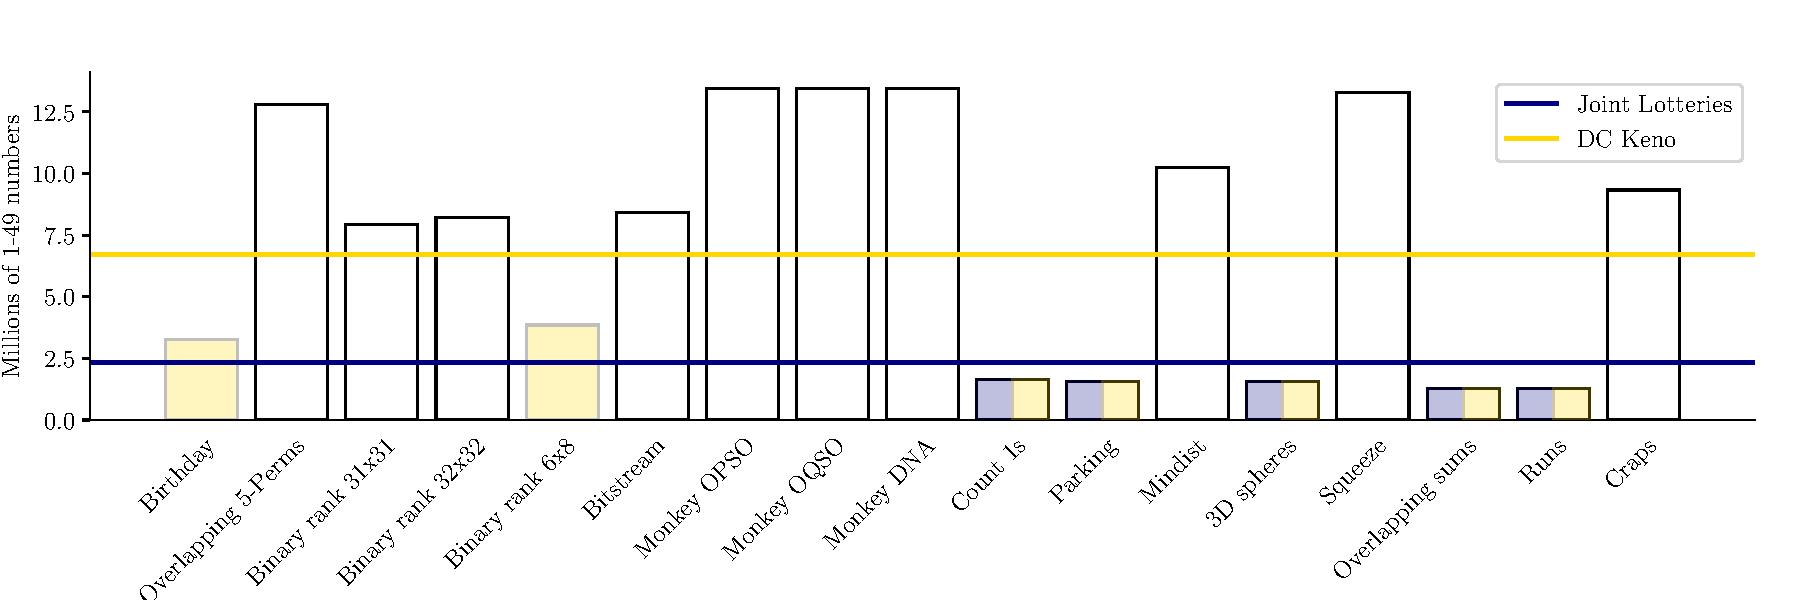
\includegraphics[width=\textwidth]{diehard_requirements.pdf}
    \caption{Amount of data required to run Diehard tests at default settings and dataset size. NY Quick Draw dataset is not present because at over 32 million numbers it falls out of scope.}
    \label{fig:requirements}
\end{figure}

\subsection{Data augmentation}

% The Diehard battery accepts a stream of bits as input. Therefore we require a function which produces uniformly distributed bit sequences from lottery numbers. To prevent any distortions to uniformity, we reject all numbers greater than 32 for 1-49 lotteries or 64 for 1-80 lotteries. We subtract one from those we keep and obtain a uniformly distributed sequence of five, respectively six bits per number. This causes a loss of about 20 \% of data, but we do not see a better way.

The Diehard tests accept streams of bits as input, so we use the binary representations of the lottery numbers.  However, we discard numbers $>$ 32 for 1-49 lotteries and $>$ 64 for 1-80 lotteries. Otherwise, the higher bits would not have equal probabilities of being active and inactive (in the 1-49 case, we would expect $\frac{17}{49} \neq \frac{1}{2}$ of the numbers to have $1$ in the highest bit). We discarded about 20 \% of our data for this reason, which exacerbated our problem of having too little data.

\subsection{Results}

There are 15 Diehard tests in the battery. All these tests operate with the null hypothesis that the data is truly random. Each of them outputs one or more p-values, which are uniformly distributed under the null hypothesis~\cite{NISTBible}. Because each test measures randomness in a different way, it is common for a single dataset to pass some tests and not others (i.e. to observe wildly different p-values for the same dataset), especially because certain tests are easier to pass than the others. An example is the Overlapping Permutations Test, which divides the sequence into subsequences of 5 and tests whether each possible subsequence occurs with equal probability. For more information on the Diehard tests, consult either the project source code or one of Marsaglia's papers~\cite{monkey,mindist}.

As a baseline, we compare our lottery datasets against randomness collected from /dev/urandom, the standard source of randomness in Linux systems~\cite{manrandom,mythsrandom}. 

% /dev/urandom represents the best source of digital randomness available to the common man and proves that the Diehard tests are working as intended.

\begin{figure}
    \centering
    \captionsetup[subfigure]{justification=centering}
    \begin{subfigure}{0.495\textwidth}
        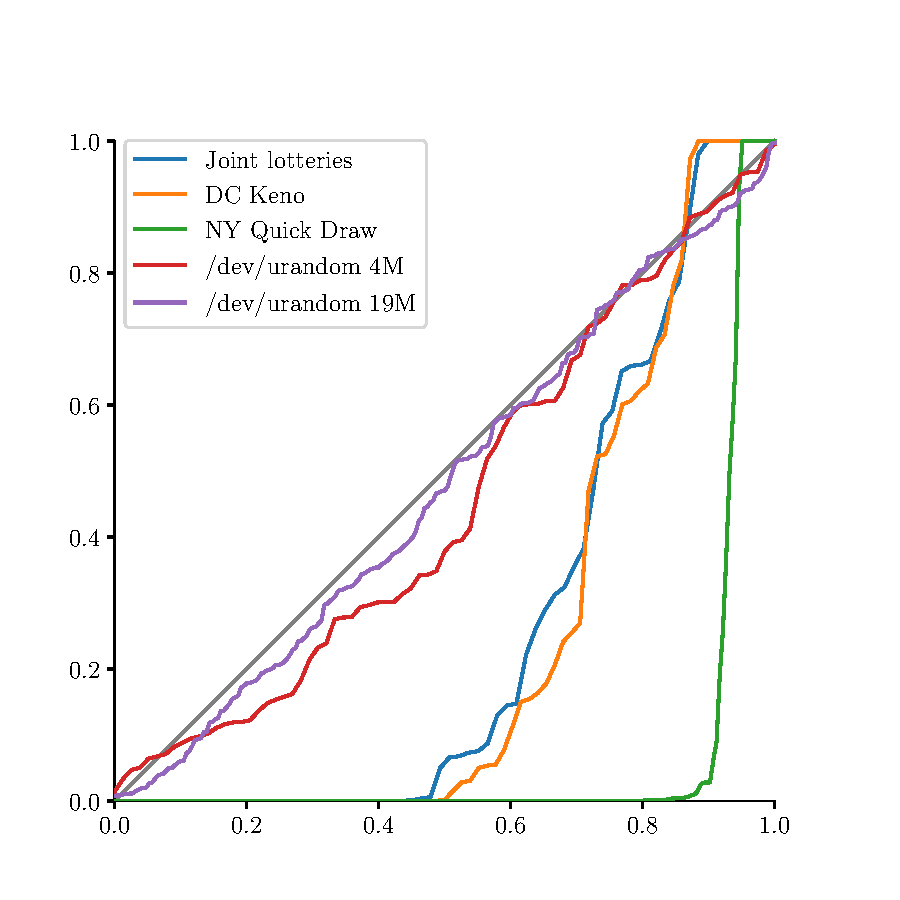
\includegraphics[width=\textwidth]{pvalue_distribution.pdf}
        \subcaption{All tests possible for each dataset.}
        \label{fig:pvalue_distribution}
    \end{subfigure}
    \hfill
    \begin{subfigure}{0.495\textwidth}
        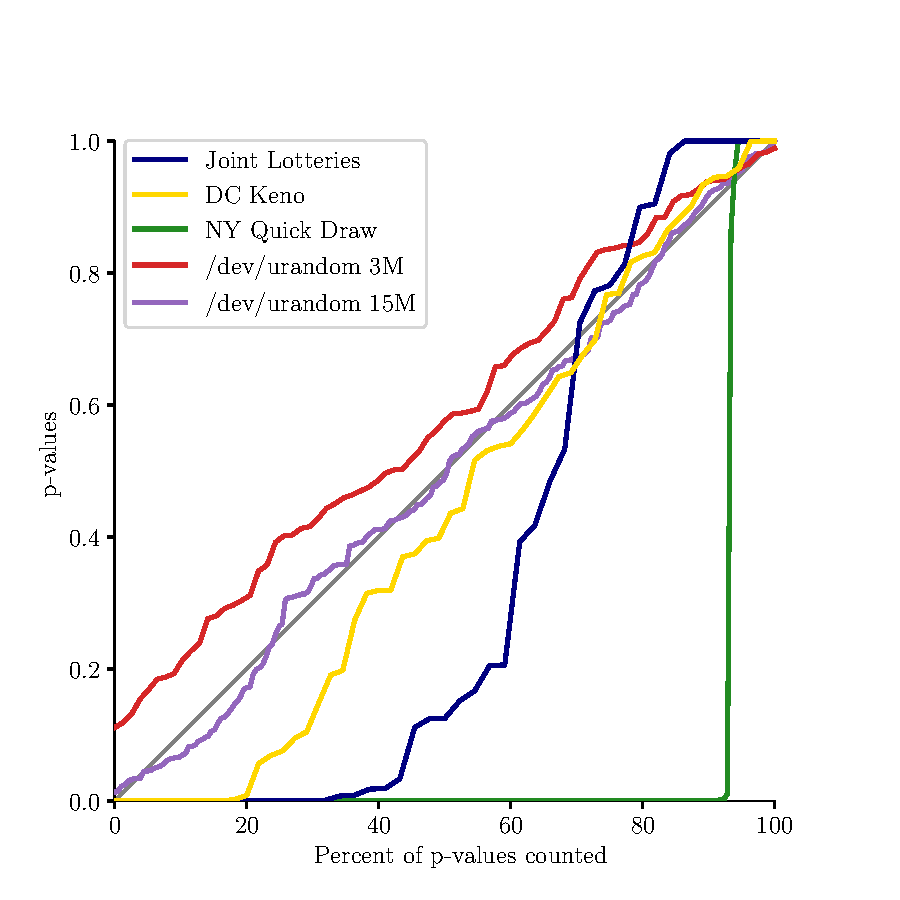
\includegraphics[width=\textwidth]{pvalue_distribution_corrected.pdf}
        \subcaption{Removed p-values from Binary Rank 6x8 test.}
        \label{fig:pvalue_corrected}
    \end{subfigure}
    \caption{Distribution of p-values for datasets. Uniform distribution of perfect randomness in gray.}
\end{figure}

We immediately notice that the NY Quick Draw catastrophically failed to pass the Diehard tests. We believe this is because the numbers are presented in sorted order, which is obviously non-random. This hypothesis is supported by the superior performance of drawn-order DC Keno dataset. In tests composed of multiple runs, the drawn-order part of Joint Lotteries dataset also results in much higher p-values than its ascending-order remainder.

The DC Keno dataset displays a remarkable even slope after it starts rising. Moreover, the 25 of the 32 zero p-values for DC Keno come from the Binary Rank 6x8 test. If we disregard this test, the resulting p-values are fairly uniformly distributed, although the dataset still struggles at some of them, corresponding to 20 \% of zero p-values. This is reasonable considering some enduring faults of the dataset (lottery drawn without replacement).

\subsection{Discussion}

There are many pitfalls to take into account. Some of them have already been addressed, such as data size, drawn/ascending order or lottery being drawn without replacement and thus not providing a truly uniform distribution.

The Diehard tests were designed to be used together as a battery. In the case of our medium-sized dataset DC Keno, we base our observations on 81 out of 213 p-values produced by the entire Diehard battery due to aforementioned size constraints. This inevitably leads to inaccuracy. We do not know how certain are our results and cannot rule out a stroke of bad luck.

Furthermore, even the Diehard battery of tests possesses flaws of its own. A critique can be found
at~\cite{dieharder, critique}. For instance, Linear Feedback Shift Registers pass the Diehard battery of tests~\cite{LFSR} despite being predictable.
